\let\negmedspace\undefined
\let\negthickspace\undefined
\documentclass[journal]{IEEEtran}
\usepackage[a5paper, margin=10mm, onecolumn]{geometry}
%\usepackage{lmodern} % Ensure lmodern is loaded for pdflatex
\usepackage{tfrupee} % Include tfrupee package

\setlength{\headheight}{1cm} % Set the height of the header box
\setlength{\headsep}{0mm}     % Set the distance between the header box and the top of the text

\usepackage{gvv-book}
\usepackage{gvv}
\usepackage{cite}
\usepackage{amsmath,amssymb,amsfonts,amsthm}
\usepackage{algorithmic}
\usepackage{graphicx}
\usepackage{textcomp}
\usepackage{xcolor}
\usepackage{txfonts}
\usepackage{listings}
\usepackage{enumitem}
\usepackage{mathtools}
\usepackage{gensymb}
\usepackage{comment}
\usepackage[breaklinks=true]{hyperref}
\usepackage{tkz-euclide} 
\usepackage{listings}
% \usepackage{gvv}                                        
\def\inputGnumericTable{}                                 
\usepackage[latin1]{inputenc}                                
\usepackage{color}                                            
\usepackage{array}                                            
\usepackage{longtable}                                       
\usepackage{calc}                                             
\usepackage{multirow} 
\usepackage{hhline}                                           
\usepackage{ifthen}                                           
\usepackage{lscape}
\usepackage{circuitikz}
\tikzstyle{block} = [rectangle, draw, fill=blue!20, 
    text width=4em, text centered, rounded corners, minimum height=3em]
\tikzstyle{sum} = [draw, fill=blue!10, circle, minimum size=1cm, node distance=1.5cm]
\tikzstyle{input} = [coordinate]
\tikzstyle{output} = [coordinate]

\begin{document}
\bibliographystyle{IEEEtran}
\vspace{3cm}

\title{MatGeo Assignment 2.6.13}
\author{AI25BTECH11007}
 \maketitle
% \newpage
% \bigskip
{\let\newpage\relax\maketitle}

\renewcommand{\thefigure}{\theenumi}
\renewcommand{\thetable}{\theenumi}
\setlength{\intextsep}{10pt} % Space between text and floats


\numberwithin{equation}{enumi}
\numberwithin{figure}{enumi}
\renewcommand{\thetable}{\theenumi}
\textbf{Question:}\\
Given that vectors $\vec{a},\vec{b},\vec{c}$ form a triangle such that
\[
\vec{a}=\vec{b}+\vec{c},
\]
find $p,q,r,s$ given that
\[
\vec{a}=p\hat{i}+q\hat{j}+r\hat{k},\qquad
\vec{b}=s\hat{i}+3\hat{j}+4\hat{k},\qquad
\vec{c}=3\hat{i}+1\hat{j}-2\hat{k},
\]
and the area of the triangle is $5\sqrt{6}$.\\


\noindent
\textbf{Solution:}\\
 We are given:

\begin{equation}
\vec{a} = \vec{b} + \vec{c}
\end{equation}

\begin{equation}
\vec{a} = p\hat{i} + q\hat{j} + r\hat{k}, \quad
\vec{b} = s\hat{i} + 3\hat{j} + 4\hat{k}, \quad
\vec{c} = 3\hat{i} + 1\hat{j} -2\hat{k}
\end{equation}

and the area of the triangle formed by these vectors is:
\begin{equation}
\text{Area} = 5\sqrt{6}
\end{equation}

\vspace{1em}
\noindent
\textbf{Observation:} For three vectors to form a triangle, they must sum to zero:
\begin{equation}
\vec{a} + \vec{b} + \vec{c} = \vec{0}
\end{equation}

However, we are told:
\begin{equation}
\vec{a} = \vec{b} + \vec{c} \Rightarrow \vec{a} - \vec{b} - \vec{c} = \vec{0}
\end{equation}

This implies:
\begin{equation}
\vec{a} + (-\vec{b}) + (-\vec{c}) = \vec{0}
\end{equation}

So, the triangle is formed by the vectors $\vec{a}, -\vec{b}, -\vec{c}$. For these to form a triangle, they must not lie along the same line (i.e., must not be collinear).

\vspace{1em}
Now, if we assume:
\begin{equation}
\vec{a} = \vec{0}
\Rightarrow \vec{b} + \vec{c} = \vec{0}
\Rightarrow \vec{b} = -\vec{c}
\end{equation}

Given:
\begin{equation}
\vec{c} = \myvec{3 \\ 1 \\ -2} 
\Rightarrow \vec{b} = -\vec{c} = -\myvec{3 \\ 1 \\ -2}
= \myvec{-3 \\ -1 \\ 2}
\end{equation}

Then:
\begin{equation}
\vec{a} = \vec{b} + \vec{c} = \vec{0}
\Rightarrow p = 0,\quad q = 0,\quad r = 0
\end{equation}

We now compute the area of the triangle using:
\begin{equation}
\text{Area} = \frac{1}{2} \left\| \vec{b} \times \vec{c} \right\|
\end{equation}

Compute the cross product:
\begin{equation}
\vec{b} \times \vec{c} = \vec{0} \Rightarrow \text{Area} = 0
\end{equation}

If we assume $\vec{a} = \vec{0}$, then $\vec{b} = -\vec{c}$, and the triangle is degenerate (i.e., the vectors lie on a straight line). Therefore, the area is zero:
\begin{equation}
\boxed{\text{Area} = 0}
\end{equation}

This contradicts the given area of $5\sqrt{6}$. Therefore, no solution exists such that:
\begin{equation}
\vec{a} = \vec{b} + \vec{c} \quad \text{and} \quad \text{Area} = 5\sqrt{6}
\end{equation}

\begin{figure}[H]
    \centering
    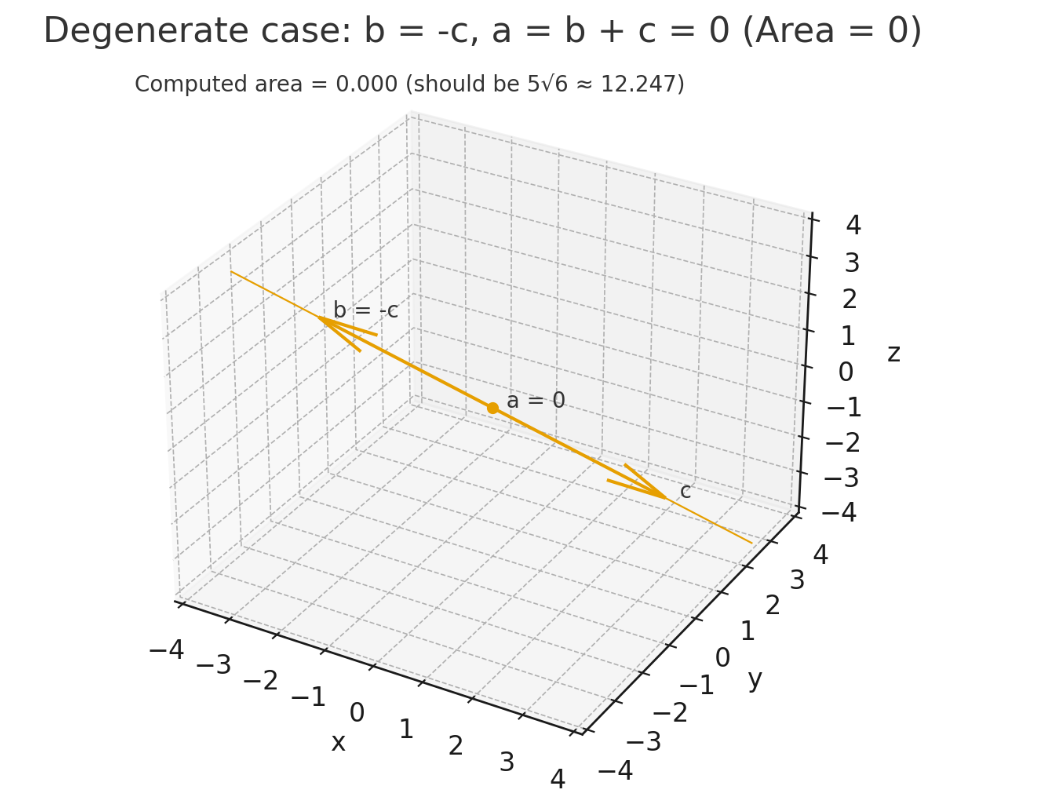
\includegraphics[width=0.75\linewidth]{figs/Screenshot 2025-09-13 191422.png}
    \caption{Image Visual}
    \label{fig:figs/Screenshot 2025-09-13 191422.png}
\end{figure}

\end{document}
